% Q19: orthographic schematic with hidden edges dashed; projection is not to scale.
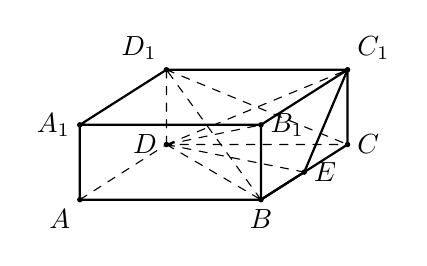
\begin{tikzpicture}[
  x={(1.15cm,0cm)},y={(0.55cm,0.35cm)},z={(0cm,0.95cm)},
  line cap=round,line join=round,>=stealth
]
  \coordinate (A) at (0,0,0);
  \coordinate (B) at (2,0,0);
  \coordinate (C) at (2,2,0);
  \coordinate (D) at (0,2,0);
  \coordinate (A1) at (0,0,1);
  \coordinate (B1) at (2,0,1);
  \coordinate (C1) at (2,2,1);
  \coordinate (D1) at (0,2,1);
  \coordinate (E) at (2,1,0);

  % Rear base edges and the rear vertical are hidden.
  \draw[dashed] (A)--(D)--(C) (D)--(D1);
  % Outer prism edges.
  \draw[thick] (A)--(B)--(C) (A)--(A1)--(B1)--(B)
    (A1)--(D1)--(C1)--(B1) (C)--(C1);
  % Spatial construction lines shown in the source sketch.
  \draw[dashed] (B)--(D1) (D)--(B1) (D)--(E) (D)--(C1) (D)--(B) (D1)--(C);
  \draw[thick] (C1)--(E) (B)--(E);

  \fill (A) circle (1pt) node[below left] {$A$};
  \fill (B) circle (1pt) node[below] {$B$};
  \fill (C) circle (1pt) node[right] {$C$};
  \fill (D) circle (1pt) node[left] {$D$};
  \fill (A1) circle (1pt) node[left] {$A_1$};
  \fill (B1) circle (1pt) node[right] {$B_1$};
  \fill (C1) circle (1pt) node[above right] {$C_1$};
  \fill (D1) circle (1pt) node[above left] {$D_1$};
  \fill (E) circle (1pt) node[right] {$E$};
\end{tikzpicture}
